\chapter{Psalm 35}

\begin{figure}
  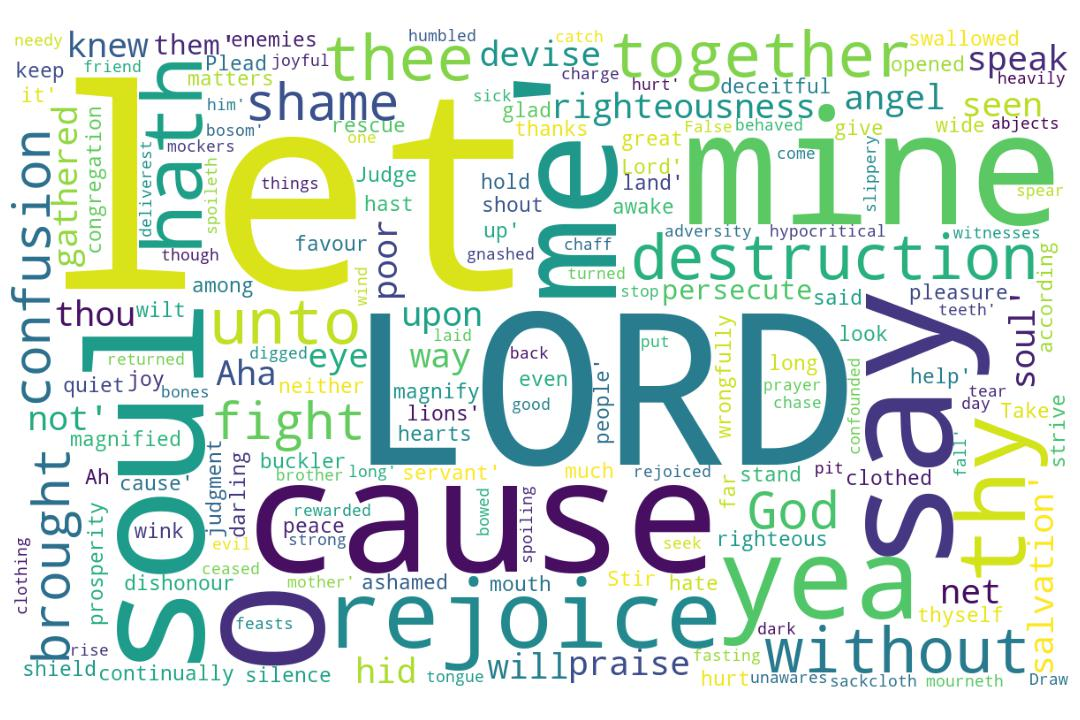
\includegraphics[width=\linewidth]{19OT-Psalms/Psalm35-WordCloud.jpg}
  \caption{Psalm 35 Word Cloud}
  \label{fig:Psalm 35 word Cloud}
\end{figure}

\marginpar{\scriptsize \centering \fcolorbox{bone}{lime}{\textbf{A HEARTFELT CRY}}\\ (Psalm 35:1--28) 
\begin{compactenum}[I.][8]
    \item A \textbf{Distinct  Petition} \index[scripture]{Psalms!Psa 035:24} (Psa 35:24)  (for enemies $\hdots$)
    \begin{compactenum}[A.][7]
		\item To be Confounded \index[scripture]{Psalms!Psa 035:04} (Psa 35:4)
		\item To be Confused \index[scripture]{Psalms!Psa 035:04}\index[scripture]{Psalms!Psa 035:26} (Psa 35:4, 26)
		\item To Become Chaff \index[scripture]{Psalms!Psa 035:05} (Psa 35:5)
		\item To be Chased \index[scripture]{Psalms!Psa 035:05} (Psa 35:5)
		\item To be Consumed \index[scripture]{Psalms!Psa 035:08} (Psa 35:8)
		\item To be Clothed in Shame \index[scripture]{Psalms!Psa 035:25} (Psa 35:25)
		\item To be Conquered \index[scripture]{Psalms!Psa 035:28} (Psa 35:28)
    \end{compactenum}
    \item A \textbf{Dangerous Prayer} \index[scripture]{Psalms!Psa 035:24} (Psa 35:24)
    \item A \textbf{Definite Promise} \index[scripture]{Psalms!Psa 035:28} (Psa 35:28)
\end{compactenum} }

\marginpar{\scriptsize \centering \fcolorbox{bone}{yellow}{\textbf{HELP, PLEASE!}}\\ (Psalm 35:1--28) 
\begin{compactenum}[I.][8]

    \item  The \textbf{Asking} \index[scripture]{Psalms!Psa 035:01} (Psa 35:1)  
    \item  \textbf{Admiration} \index[scripture]{Psalms!Psa 035:10} (Psa 35:10)  
    \item  \textbf{Adversity} \index[scripture]{Psalms!Psa 035:15} (Psa 35:15)  
    \item  \textbf{Abjects} \index[scripture]{Psalms!Psa 035:15} (Psa 35:15)  
    \item  \textbf{Adversaries} \index[scripture]{Psalms!Psa 035:15} (Psa 35:15)  
    \item  \textbf{Assembly} \index[scripture]{Psalms!Psa 035:18} (Psa 35:18)  
    \item  \textbf{Activation} \index[scripture]{Psalms!Psa 035:23} (Psa 35:23)  
    \item  \textbf{Acknowledgment} \index[scripture]{Psalms!Psa 035:27} (Psa 35:27)  
\end{compactenum} }

%%%%%%%%%%%%%%%%%%%%%%%%%%%%%%%%%%%%%%%%%%%%%%
%%%%%%%%%%%%%%%%%%%%%%%%%%%%%%%%%%%%%%%%%%%%%%
\footnote{\textcolor[cmyk]{0.99998,1,0,0}{\hyperlink{TOC}{Return to end of Table of Contents.}}}\footnote{\href{https://audiobible.com/bible}{\textcolor[cmyk]{0.99998,1,0,0}{Psalms Audio}}}\textcolor[cmyk]{0.99998,1,0,0}{Plead \emph{my} \emph{cause}, O LORD, with them that strive with me: fight against them that fight against me.}\marginpar{\scriptsize \textcolor[rgb]{0.00,0.545,0.269}{$\rightarrow$(1) Strife [1], (2) Shield [2], (3) Spear [3], (4) Salvation [3], (5) Shame [4], (6) Slipping [6], (7) Spoiling [10].}}
[2] \textcolor[cmyk]{0.99998,1,0,0}{Take hold of shield and buckler, and stand up for mine help.}
[3] \textcolor[cmyk]{0.99998,1,0,0}{Draw out also the spear, and stop \emph{the} \emph{way} against them that persecute me: say unto my soul, I \emph{am} thy salvation.}
[4] \textcolor[cmyk]{0.99998,1,0,0}{Let them be \fcolorbox{bone}{lime}{confounded} and put to shame that seek after my soul: let them be turned back and brought to \fcolorbox{bone}{lime}{confusion} that devise my hurt.}
[5] \textcolor[cmyk]{0.99998,1,0,0}{Let them be as \fcolorbox{bone}{lime}{chaff} before the wind: and let the angel of the LORD \fcolorbox{bone}{lime}{chase} \emph{them}.}
[6] \textcolor[cmyk]{0.99998,1,0,0}{Let their way be dark and slippery: and let the angel of the LORD persecute them.}
[7] \textcolor[cmyk]{0.99998,1,0,0}{For without cause have they hid for me their net \emph{in} a pit, \emph{which} without cause they have digged for my soul.}
[8] \textcolor[cmyk]{0.99998,1,0,0}{Let \fcolorbox{bone}{lime}{destruction} come upon him at unawares; and let his net that he hath hid catch himself: into that very destruction let him fall.}
[9] \textcolor[cmyk]{0.99998,1,0,0}{And my soul shall be joyful in the LORD: it shall rejoice in his salvation.}
[10] \textcolor[cmyk]{0.99998,1,0,0}{All my bones shall say, LORD, who \emph{is} like unto thee, which deliverest the poor from him that is too strong for him, yea, the poor and the needy from him that spoileth him?}
[11] \textcolor[cmyk]{0.99998,1,0,0}{False witnesses did rise up; they laid to my charge \emph{things} that I knew not.}
[12] \textcolor[cmyk]{0.99998,1,0,0}{They rewarded me evil for good \emph{to} the spoiling of my soul.}
[13] \textcolor[cmyk]{0.99998,1,0,0}{But as for me, when they were sick, my clothing \emph{was} sackcloth: I humbled my soul with fasting; and my prayer returned into mine own bosom.}
[14] \textcolor[cmyk]{0.99998,1,0,0}{I behaved myself as though \emph{he} \emph{had} \emph{been} my friend \emph{or} brother: I bowed down heavily, as one that mourneth \emph{for} \emph{his} mother.}
[15] \textcolor[cmyk]{0.99998,1,0,0}{But in mine adversity they rejoiced, and gathered themselves together: \emph{yea}, the abjects gathered themselves together against me, and I knew \emph{it} not; they did tear \emph{me}, and ceased not:}
[16] \textcolor[cmyk]{0.99998,1,0,0}{With hypocritical mockers in feasts, they gnashed upon me with their teeth.}
[17] \textcolor[cmyk]{0.99998,1,0,0}{Lord, how long wilt thou look on? rescue my soul from their destructions, my darling from the lions.}
[18] \textcolor[cmyk]{0.99998,1,0,0}{I will give thee thanks in the great congregation: I will praise thee among much people.}
[19] \textcolor[cmyk]{0.99998,1,0,0}{Let not them that are mine enemies wrongfully rejoice over me: \emph{neither} let them wink with the eye that hate me without a cause.}
[20] \textcolor[cmyk]{0.99998,1,0,0}{For they speak not peace: but they devise deceitful matters against \emph{them} \emph{that} \emph{are} quiet in the land.}
[21] \textcolor[cmyk]{0.99998,1,0,0}{Yea, they opened their mouth wide against me, \emph{and} said, Aha, aha, our eye hath seen \emph{it}.}
[22] \textcolor[cmyk]{0.99998,1,0,0}{\emph{This} thou hast seen, O LORD: keep not silence: O Lord, be not far from me.}
[23] \textcolor[cmyk]{0.99998,1,0,0}{Stir up thyself, and awake to my judgment, \emph{even} unto my cause, my God and my Lord.}
[24] \textcolor[cmyk]{0.99998,1,0,0}{\fcolorbox{bone}{lime}{Judge me}, O LORD my God, according to thy righteousness; and let them not rejoice over me.}
[25] \textcolor[cmyk]{0.99998,1,0,0}{Let them not say in their hearts, Ah, so would we have it: let them not say, We have swallowed him up.}
[26] \textcolor[cmyk]{0.99998,1,0,0}{Let them be ashamed and brought to confusion together that rejoice at mine hurt: let them be clothed with shame and dishonour that magnify \emph{themselves} against me.}
[27] \textcolor[cmyk]{0.99998,1,0,0}{Let them shout for joy, and be glad, that favour my righteous cause: yea, let them say continually, Let the LORD be magnified, which hath pleasure in the prosperity of his servant.}
[28] \textcolor[cmyk]{0.99998,1,0,0}{And my tongue \fcolorbox{bone}{lime}{shall speak} of thy righteousness \emph{and} of thy praise all the day long.}


